\section{High Energy}
\subsection{Questions}
\begin{enumerate}
\item \textbf{Describe the mechanisms by which cosmic rays gain and lose energy. Which mechanisms
      are appropriate to which type of particle? Which ones produce electromagnetic
      radiation that we can observe, and in what wave bands?}
\item \textbf{Discuss the equation of state of relativistic/nonrelativistic degenerate gases of electrons
      and neutrons and derive the Chandrasekhar mass limit for white dwarfs. (A
      heuristic approach, as in Shapiro and Teukolsky, is sufficient.)}
      
      Let's derive the degeneracy pressure for nonrelativistic electrons. First we look at the Heisenberg uncertainty principle, which states that $\Delta x \Delta p \ge \frac{h}{2\pi}$. Therefore the minimum phase space that can be occupied by two electrons is $\Delta x \Delta y \Delta z \Delta p_x \Delta p_y \Delta p_z \sim h^3$ (don't ask me why there isn't a factor of $8 \pi^3$ on the bottom, but no one puts it in). The density $n(p) = 2/h^3$, since two electrons can occupy each cell of $h^3$ space. To get the spatial electron density, integrate over momentum:
      \begin{equation}
      n_e = \int_0^{p_F} 4\pi p^2 dp = \frac{8 \pi}{3 h^3} p_F^3\,\,,
      \end{equation}
      where we have assumed that at $T=0$ (or rather that thermal pressure is very small compared to degeneracy pressure, the maximum momentum is the Fermi momentum. We now know that
      \begin{equation}
      p_F = \biggl( \frac{3 h^3}{8 \pi} n_e \biggr) ^{1/3}
      \end{equation}
      and
      \begin{equation}
      E_F = \frac{p_F^2}{2m_e} = \biggl( \frac{3 h^3}{8 \pi} n_e \biggr) ^{2/3}\frac{1}{2m_e}\,\,.
      \end{equation}
      
      Now let's figure out how to get the pressure. %Define the phase space distribution $\tilde{f} = \frac{g_s}{h^3} f$, where $g_s = 2S + 1$ which is $2$ in the case of spin-1/2 particles. The pressure is defined by
      \begin{equation}
      P = \frac{1}{3} \int p v n(p) 4 \pi p^2 dp\,\,.
      \end{equation}
      We also know the electron density
      \begin{equation}
      n_e = \frac{\rho}{\mu_e m_H},~\mu_e = \frac{A}{Z} \approx 2
      \end{equation}
      for a regular white dwarf. Now let's calculate the electron degeneracy pressure in the nonrelativistic case, in which $v = p/m_e$. Then we have
      \begin{equation}
      P_e = \frac{1}{3} \int^{p_F}_0 p \frac{p}{m_e} \frac{2}{h^3} 4 \pi p^2 dp = \frac{8 \pi p_F^5}{15 h^3 m_e}\,\,.
      \end{equation}
      Plugging in for $p_F$ gives
      \begin{equation}
      P_e = \frac{8\pi}{15 h^3 m_e} \biggl( \frac{3 h^3 \rho}{8 \pi\mu_e m_H}\biggr)^{5/3} = \frac{h^2}{5 m_e} \biggl( \frac{3}{8 \pi} \biggr)^{2/3}\biggl( \frac{\rho}{\mu_e m_H} \biggr)^{5/3}\,\,.
      \end{equation}
      You can simplify this further and make it pretty, but the important thing is that this has the form $P_e = k_1 \rho^{5/3}$, so it follows an adiabatic form of the pressure. It's also convenient to write this as $P_e = k_1^\prime \biggl( \frac{\rho}{\mu_e} \biggr)^{5/3}$ so the degeneracy pressure depends on both the density and the electron fraction of the gas. If there are nuclear reactions going on, $\mu_e$ may change and $k_1$ will not be constant.
      
      Now let's look at the very relativistic case. Here we can approximate $v \sim c$, and the pressure becomes
      \begin{equation}
      P_{e,r} = \frac{1}{3} \int^{p_F}_0 p c \frac{2}{h^3} 8 \pi p^2 dp = \frac{8\pi c p_F^4}{12 h^3} = \frac{2\pi c p_F^4}{3 h^3}\,\,.
      \end{equation}
      This can be rewritten as
      \begin{equation}
      P_{e,r} = \frac{2\pi c}{3 h^3} \biggl( \frac{3 h^3 \rho}{8 \pi\mu_e m_H} \biggr)^{4/3} = \frac{h c}{4} \biggl(\frac{3}{8 \pi}\biggr)^{1/3} \biggl(\frac{\rho}{\mu_e m_H}\biggr)^{4/3}
      \end{equation}
      This we can rewrite as $P_{e,r} = k_2 \rho^{4/3} = k_2^\prime \biggl(\frac{\rho}{\mu_e}\biggr)^{4/3}$, so this is also a polytrope but with adiabatic index $4/3$. We will see in a second that this is key to showing that white dwarfs have a maximum mass once their electrons become ultrarelativistic.
      
      Off the top of my head, I don't know how to derive this rigorously, but for now here's a hand-wavey version. Use the relativistic electron degeneracy pressure and hydrostatic equilibrium, which we will wave into this form:
      \begin{equation}
      \frac{P}{R} \sim \frac{G M \rho}{R^2} \sim \frac{3 G M^2}{4 \pi R^5}\,\,.
      \end{equation}
      Set this equal to our adiabatic pressure to get
      \begin{equation}
      P \approx \frac{3 G M^2}{4 \pi R^4} \sim k_2 \rho^{4/3} \approx k_2 \biggl(\frac{3 M}{4 \pi R^3}\biggr)^{4/3}\,\,.
      \end{equation}
      Rearranging, we get
      \begin{equation}
      M^{2/3} \approx \biggl(\frac{4\pi}{3 G} \biggr)\biggl(\frac{2\pi c}{2 h^3} \biggr)\biggl(\frac{3 h^3}{8 \pi \mu_e m_H} \biggr)^{4/3} \biggl(\frac{3}{4 \pi} \biggr)^{4/3}
      \end{equation}
      Note that this formula for the mass is all constants (assuming $\mu_e$ doesn't change)! That means mass no longer scales with radius or anything else, and we have found a unique mass at which electrons must travel at the speed of light in order to support it. The numbers work out to give $3.077 \times 10^{32}~{\rm g}$. This is off by a factor of 10 from the value we want... can someone check my work? maybe I shouldn't hand-wave.
      
\item \textbf{Derive the equation for the effective temperature of an accretion disk around a
      black hole of mass $M$ with accretion rate $\dot M$, as a function of radius $r$. Specify the
      assumptions required to get an answer, and comment on what could go wrong with
      them. Define the Eddington luminosity and explain its relevance to the peak frequency
      of the emitted radiation.}
      
      Consider the vertical structure of an accretion disk, assume we're at large radii ($r \gg r_{\rm in}$), and assume it's a thin disk radiating mostly just through the top and bottom. The heating rate per volume is
      \begin{equation}
      \nabla \cdot F_{\rm rad} = \rho \nu (r \Omega^\prime)^2 = \rho \nu \biggl(\frac{3}{2} \Omega \biggr)^2
      \end{equation}
      from assuming that the rotation is Keplerian. Use radiative diffusion with $P_{\rm rad} = \frac{1}{3} a T^4 = \frac{1}{3}\frac{4 \sigma_{\rm SB}}{c}T^4$. Assume that the disk is optically thick enough that the spectrum is a blackbody. Assume radiation travelling through a layer that is one mean free path $\lambda = 1/\kappa \rho$ thick is what's giving you the flux. The flux is then the speed of light times the mean free path times the change in radiation pressure with height (note: I have not totally justified this expression. If anyone can shed light on this, that'll be cool):
      \begin{equation}
      F_{\rm rad} - \frac{1}{\kappa \rho} \frac{d}{dz}P_{\rm rad} c = -\frac{4}{3}\frac{\sigma_{\rm SB}}{\kappa \rho}\frac{\partial T^4}{\partial z}
      \end{equation}
      This is similar to the radiative diffusion equation for stars\footnote{$L(r) = -4 \pi r^2 \frac{4}{3} \frac{c a T^3}{\kappa\rho}\frac{\partial T}{\partial r}$}. Now let's integrate vertically, because we want the total flux from each vertical layer in the accretion disk coming out of the top and bottom of the disk.
      \begin{equation}
      \int^\infty_0 \frac{\partial F_{\rm rad}}{\partial z} = \sigma T_{\rm eff}^4 = \frac{1}{2} \Sigma \langle \nu \rangle \frac{9}{4}\Omega^2 = \frac{9}{8} \frac{G M \dot{M}}{3 \pi r^3}
      \end{equation}
      Now approximate 
      \begin{equation}
      -\frac{4}{3} \frac{\sigma_{\rm SB}}{\kappa rho} \frac{\partial T^4}{\partial z} \approx D(r) = \frac{3}{8 \pi}\frac{GM\dot{M}}{r^3}\biggl[1 - \sqrt{\frac{r_{\rm in}}{r}} \biggr]
      \end{equation}
      
      We eventually want to get here:
      \begin{equation}
      D(r) \approx \frac{4}{3}\frac{\sigma_{\rm SB}}{\kappa \rho}\frac{T^4_{\rm midplane}}{H} \approx \frac{4}{3}\sigma_{\rm SB}\frac{T^4_{\rm midplane}}{\tau_{\rm vert}} = \frac{4}{3}\sigma_{\rm SB}T^4_{\rm eff}
      \end{equation}
      
      
\end{enumerate}

\subsection{Fluids and the Sonic Point}

For reference, here is the general equation for accretion and winds for which you have a steady state, that is, $\dot{M} = 4 \pi r^2 \rho v$ is a constant with radius:

\begin{equation}
\frac{1}{v} \frac{dv}{dr} (v^2 - c_s^2) = \frac{2 c_s^2}{r} - \frac{G M}{r^2}\,\,.
\end{equation}
Solutions are depicted in Figure \ref{f:mach}. The point where $v = c_s$ is called the sonic point, and it represents the transition between subsonic and supersonic flow.

\subsection{White Dwarfs}

\subsection{Supernovae}

\subsection{Neutron Stars}

\subsection{Black Holes}


\subsection{Bondi Accrection}

Bondi accrection, also called spherical accretion, assumes your central object of mass $M$ is accreting isotropically from an ambient medium at infinity with density $\rho_\infty$, temperature $T_\infty$, $v_\infty = 0$, and sound speed $c_{s\infty}^2$. We're looking for a steady state solution, so $\nabla \cdot (\rho \underline{v}) = 0$ and $\frac{1}{2} v^2 + \phi + h = {\rm constant}$, which is Bernoulli's constant. Here, $\phi = \frac{-G M}{r}$, so we're neglecting self-gravity of the accreting fluid. We also have
\begin{equation}
h = \epsilon + \frac{P}{\rho} = \frac{1}{\Gamma - 1}\frac{P}{\rho} + \frac{P}{\rho} = \frac{c_s^2}{\Gamma - 1}\,\, ,
\end{equation}
where $\Gamma = 5/3$ for monatomic gas. Let's define the Bondi radius, which separates regimes where gravity is and is not dominant:
\begin{equation}
r_B = \frac{G M}{c_{s \infty}^2} \,\,.
\end{equation}
Now let's use Bernoulli's equation to relate the quantities when the gas is at infinity to the quantities at some radius $r$:
\begin{equation}
\frac{1}{2} v_r^2 - \frac{G M}{r} + \frac{1}{\Gamma - 1} c_s^2(r) = \frac{1}{\Gamma - 1} c_{s \infty}^2
\end{equation}
since at infinity, both $v_r$ and $\phi$ go to zero. Dividing out $c_{s \infty}^2$, this equation can be rewritten as 
\begin{equation}
\frac{1}{2}\frac{v_r^2(r)}{c_s^2(r)}\frac{c_s^2(r)}{c_{s \infty}^2(r)} - \frac{r_B}{r} + \frac{1}{\Gamma - 1}\frac{c_s^2(r)}{c_{s \infty}^2(r)} = \frac{1}{\Gamma - 1}
\end{equation}
Let's define here the Mach number $\mathcal{M} = \frac{v_r^2(r)}{c_s^2(r)}$. Also write $\rho_* = \frac{\rho}{\rho_\infty}$, and this equation becomes
\begin{equation}
\frac{\Gamma - 1}{2}\mathcal{M}^2 \rho_*^{\Gamma - 1} + \rho_*^{\Gamma - 1} = 1 + \frac{\Gamma - 1}{r_*}\,\, ,
\end{equation}
where $r_* = r/r_B$. We can use the fact that $4 \pi r^2 \rho v_r = \dot{M}$ is a constant with radius to eventually solve for the Mach number as a function of radius. There are lines of solutions, which matter will follow (some are not physical), shown in Figure \ref{f:mach}. The solutions that cross the sonic point ($\mathcal{M} = 1$) represent physical accretion and wind solutions. The descending curve is for accretion, and the ascending curve is for a wind that goes supersonic.

\begin{figure}[!h]
\begin{center}
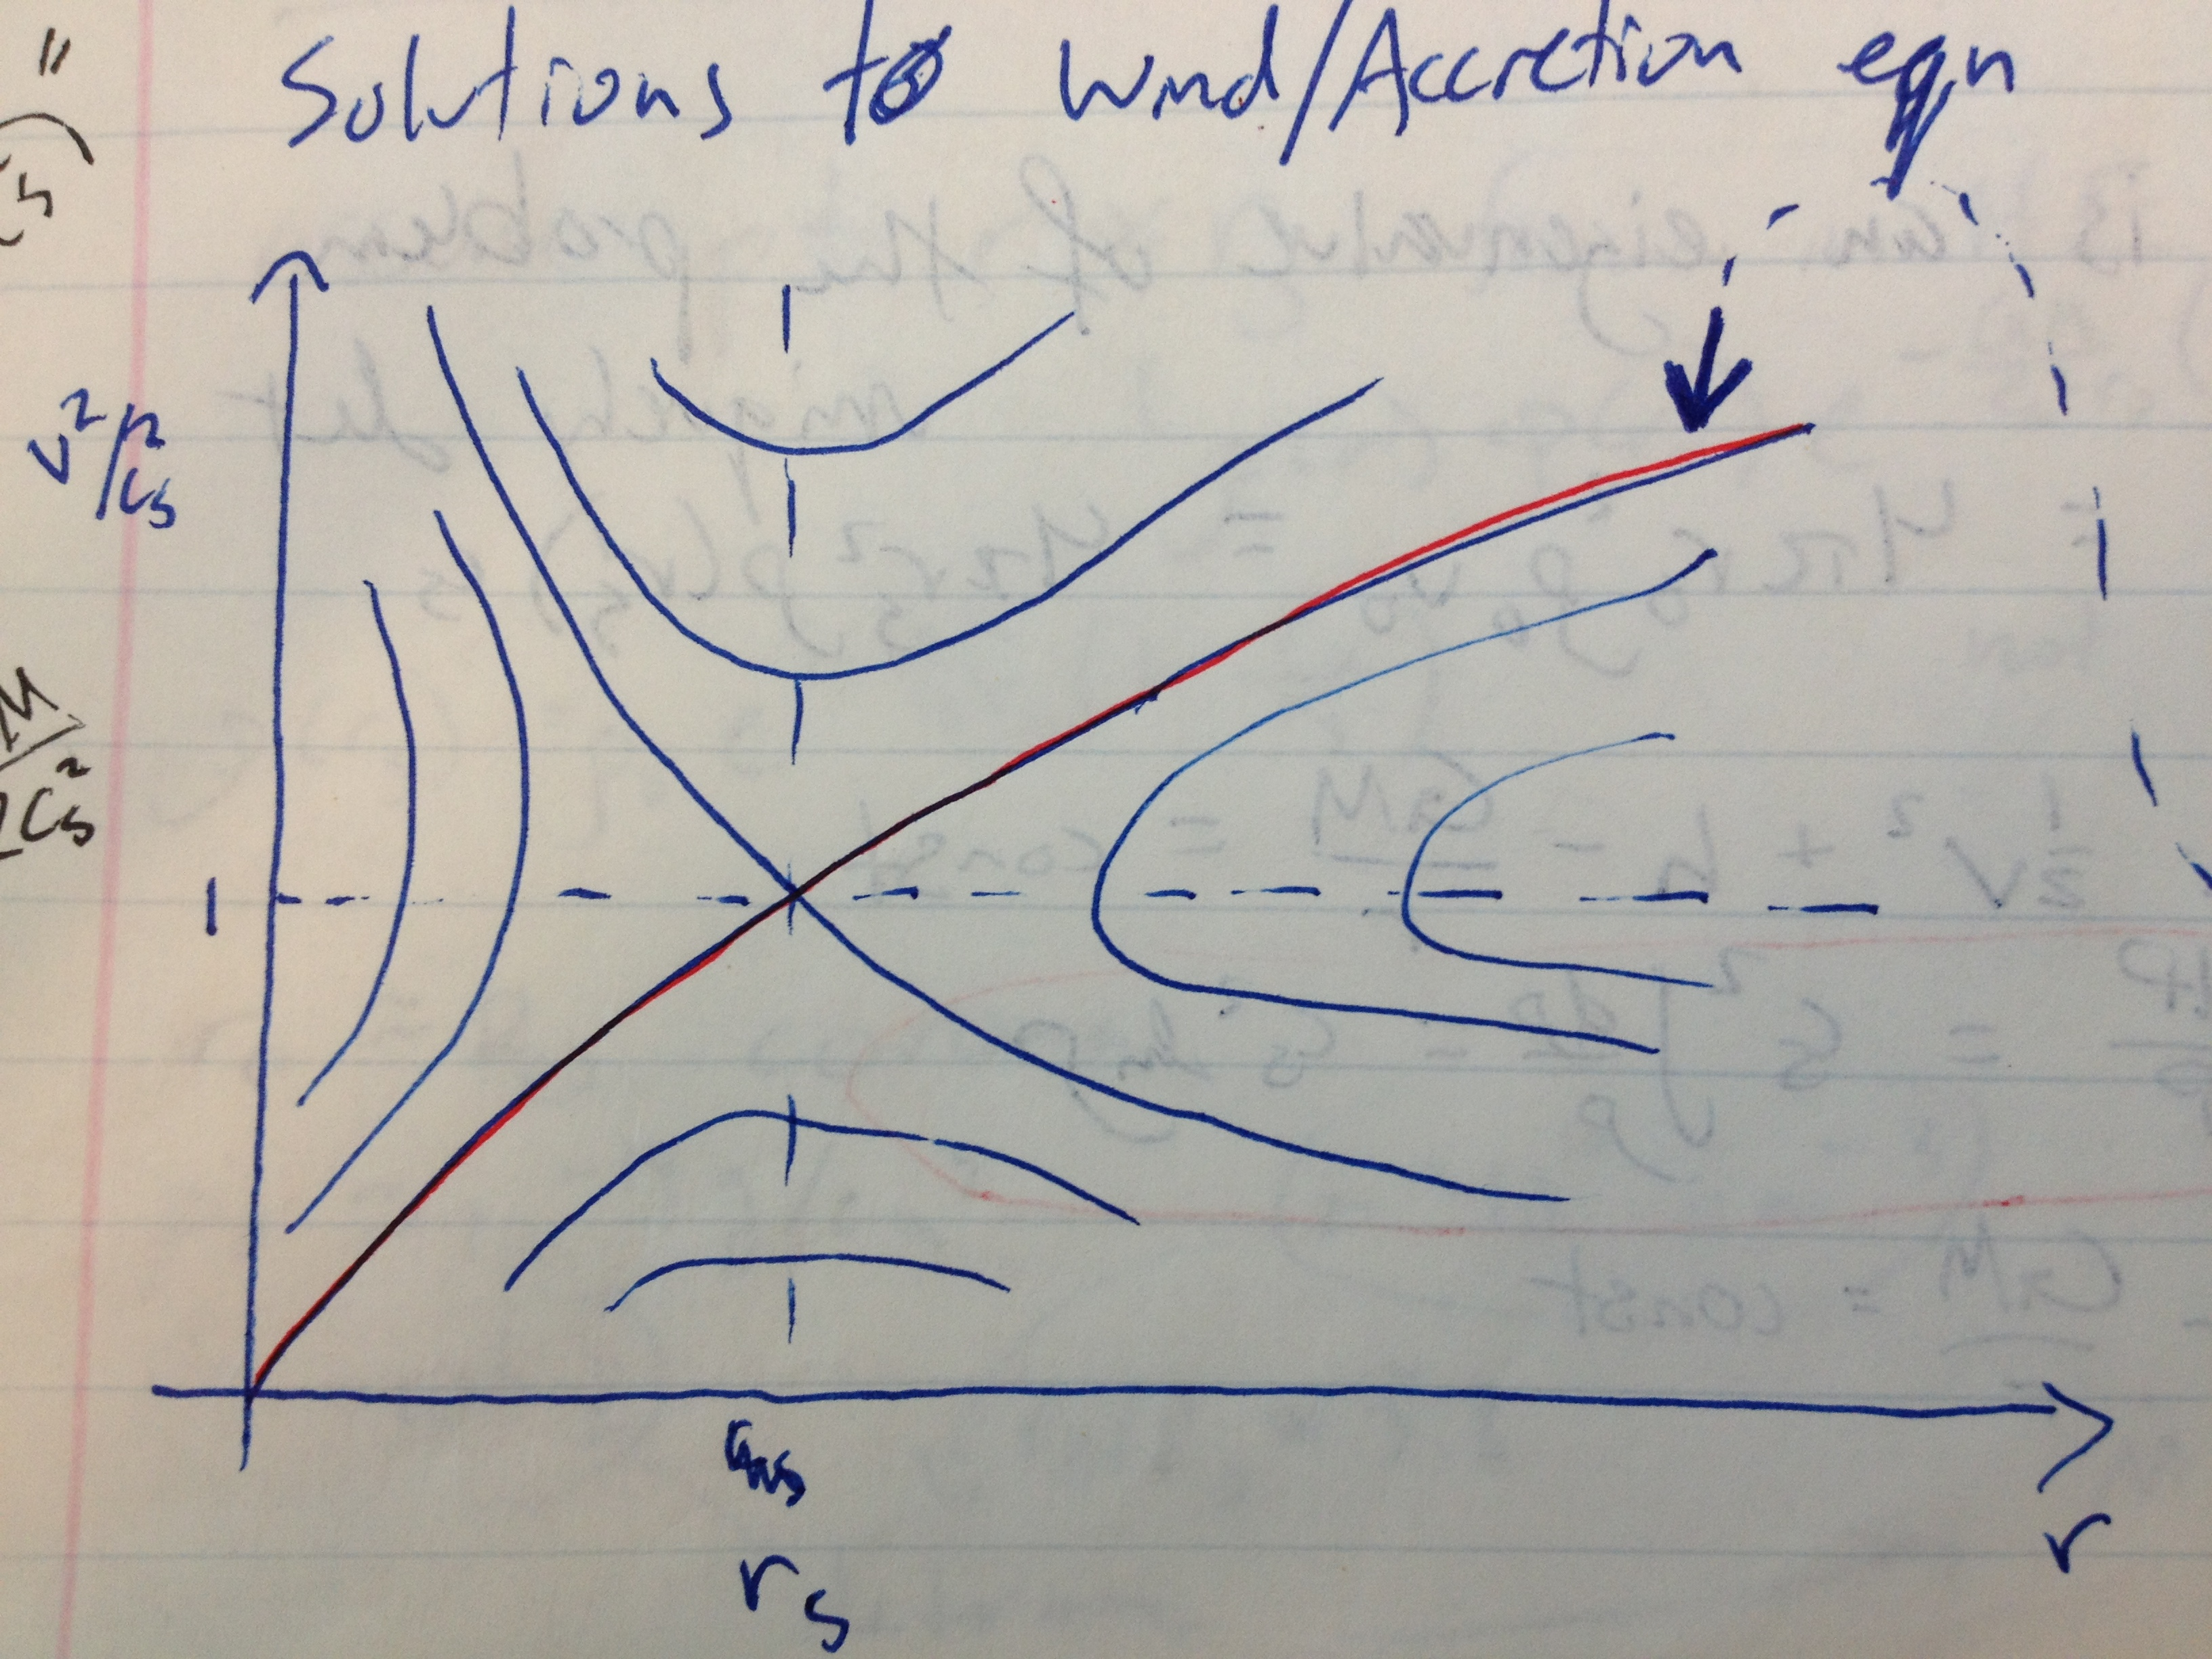
\includegraphics[width=\textwidth]{mach.jpg}
\caption{Mach number as a function of radius showing wind and accretion solutions \label{f:mach}}
\end{center}
\end{figure}

The sonic transition can be used to uniquely define $\dot{M}$:
\begin{equation}
\dot{M} = \lambda 4 \pi \biggl( \frac{G M}{c_{s \infty}^2} \biggr) ^2 \rho_\infty c_{s \infty}\,\, ,
\end{equation}
where $\lambda$ depends on $\Gamma$ and is $0.25$ for $\Gamma = 5/3$, $0.71$ for $\Gamma = 4/3$, $1.12$ for $\Gamma = 1$.

Let's also look at Bondi-Hoyle accretion, which is similar to Bondi accretion, except it's for a mass that's moving through the stuff it's accreting. This time, we can approximate:
\begin{equation}
\dot{M} = \pi \biggl(\frac{2 G M}{v_\infty ^2 + c_{s \infty}^2} \biggr)^2 \rho_* \sqrt{v_\infty ^2 + c_{s \infty}^2}\,\, .
\end{equation}
In this case, the incoming gas (from the perspective of the accreting mass) travels around the object and meets on the other side. This creates a shock in the gas, which heats and expands, and eventually this creates a bow shock around the accreting object as it moves through the fluid.

\subsection{Accretion Disks}

The idea behind accretion disks is that material falls in and maintains the angular momentum it had at large radii, so it starts to orbit the central mass. Viscosity in the disk is what causes it to heat up and radiate, which causes the material to lose energy and start falling in. Let's assume an axisymmetric situation. For Keplertian rotation, $v_\phi = \sqrt{\frac{GM}{r}}$. Because the velocity decreases with radius, we can imagine a thin ring of the disk with an adjacent interior ring moving more slowly and an adjacent outer ring moving more quickly. Imagine elements in these three rings for temporary `bonds' with each other, so the inner ring gets pulled back and bit and the outer ring gets pushed forward a bit due to the interaction between the rings (which is due to viscosity). Actually, the lowest energy state that the disk is trying to get to is one in which a small part of the mass goes out to infinity and carries all the angular momentum with it, while the rest of the accretion disk falls into the accretor.

One good thing to know about an accretion disk is its thickness. The scale height $H$ provides a measure of the thickness when compared with the radius $R$. It's possible to approximate the scale height by using hydrostatic equilibrium in the $z$ direction:
\begin{equation}
\frac{dP}{dz} = -g_z \rho = -\frac{GM}{r^2} \frac{z}{r}\,\,.
\end{equation}
We can hand-wave this by setting $dz = z = H$ and $r = R$ and using ideal gas for $P$:
\begin{equation}
H \sim \biggl( \frac{k_{\rm B} T R^3}{GM m_p}\biggr)^{1/2}\,\,.
\end{equation}
Typical temperatures are around $10^4~{\rm K}$.

Now let's define the surface mass density $\Sigma(r) = \int^\infty_{-\infty} \rho dz$. We can get the average velocity $\langle v_r \rangle$ by integrating $v_r$ over $z$ and $\phi$ in a mass-weighted way. Then we can get the accretion rate,
\begin{equation}
\dot{M} = 2 \pi r \Sigma \langle v_r \rangle\,\, ,
\end{equation}
which is constant with $r$.

Let's look at energy dissipation in the disk. First define the shear $\sigma_{\hat{r}\hat{\phi}} = \frac{1}{2}(v_{x,y} + v_{y,x})$.

(note: I am having trouble condensing this into the important information about accretion disks. If anyone wants to add and restructure, go for it. I'll work on some other things and come back to it later. -io)

\subsection{High-Energy Binaries}

\subsection{GRBs}

\subsection{AGN}

\subsection{Cosmic Rays}
